\documentclass[1p]{elsarticle_modified}
%\bibliographystyle{elsarticle-num}

%\usepackage[colorlinks]{hyperref}
%\usepackage{abbrmath_seonhwa} %\Abb, \Ascr, \Acal ,\Abf, \Afrak
\usepackage{amsfonts}
\usepackage{amssymb}
\usepackage{amsmath}
\usepackage{amsthm}
\usepackage{scalefnt}
\usepackage{amsbsy}
\usepackage{kotex}
\usepackage{caption}
\usepackage{subfig}
\usepackage{color}
\usepackage{graphicx}
\usepackage{xcolor} %% white, black, red, green, blue, cyan, magenta, yellow
\usepackage{float}
\usepackage{setspace}
\usepackage{hyperref}

\usepackage{tikz}
\usetikzlibrary{arrows}

\usepackage{multirow}
\usepackage{array} % fixed length table
\usepackage{hhline}

%%%%%%%%%%%%%%%%%%%%%
\makeatletter
\renewcommand*\env@matrix[1][\arraystretch]{%
	\edef\arraystretch{#1}%
	\hskip -\arraycolsep
	\let\@ifnextchar\new@ifnextchar
	\array{*\c@MaxMatrixCols c}}
\makeatother %https://tex.stackexchange.com/questions/14071/how-can-i-increase-the-line-spacing-in-a-matrix
%%%%%%%%%%%%%%%

\usepackage[normalem]{ulem}

\newcommand{\msout}[1]{\ifmmode\text{\sout{\ensuremath{#1}}}\else\sout{#1}\fi}
%SOURCE: \msout is \stkout macro in https://tex.stackexchange.com/questions/20609/strikeout-in-math-mode

\newcommand{\cancel}[1]{
	\ifmmode
	{\color{red}\msout{#1}}
	\else
	{\color{red}\sout{#1}}
	\fi
}

\newcommand{\add}[1]{
	{\color{blue}\uwave{#1}}
}

\newcommand{\replace}[2]{
	\ifmmode
	{\color{red}\msout{#1}}{\color{blue}\uwave{#2}}
	\else
	{\color{red}\sout{#1}}{\color{blue}\uwave{#2}}
	\fi
}

\newcommand{\Sol}{\mathcal{S}} %segment
\newcommand{\D}{D} %diagram
\newcommand{\A}{\mathcal{A}} %arc


%%%%%%%%%%%%%%%%%%%%%%%%%%%%%5 test

\def\sl{\operatorname{\textup{SL}}(2,\Cbb)}
\def\psl{\operatorname{\textup{PSL}}(2,\Cbb)}
\def\quan{\mkern 1mu \triangleright \mkern 1mu}

\theoremstyle{definition}
\newtheorem{thm}{Theorem}[section]
\newtheorem{prop}[thm]{Proposition}
\newtheorem{lem}[thm]{Lemma}
\newtheorem{ques}[thm]{Question}
\newtheorem{cor}[thm]{Corollary}
\newtheorem{defn}[thm]{Definition}
\newtheorem{exam}[thm]{Example}
\newtheorem{rmk}[thm]{Remark}
\newtheorem{alg}[thm]{Algorithm}

\newcommand{\I}{\sqrt{-1}}
\begin{document}

%\begin{frontmatter}
%
%\title{Boundary parabolic representations of knots up to 8 crossings}
%
%%% Group authors per affiliation:
%\author{Yunhi Cho} 
%\address{Department of Mathematics, University of Seoul, Seoul, Korea}
%\ead{yhcho@uos.ac.kr}
%
%
%\author{Seonhwa Kim} %\fnref{s_kim}}
%\address{Center for Geometry and Physics, Institute for Basic Science, Pohang, 37673, Korea}
%\ead{ryeona17@ibs.re.kr}
%
%\author{Hyuk Kim}
%\address{Department of Mathematical Sciences, Seoul National University, Seoul 08826, Korea}
%\ead{hyukkim@snu.ac.kr}
%
%\author{Seokbeom Yoon}
%\address{Department of Mathematical Sciences, Seoul National University, Seoul, 08826,  Korea}
%\ead{sbyoon15@snu.ac.kr}
%
%\begin{abstract}
%We find all boundary parabolic representation of knots up to 8 crossings.
%
%\end{abstract}
%\begin{keyword}
%    \MSC[2010] 57M25 
%\end{keyword}
%
%\end{frontmatter}

%\linenumbers
%\tableofcontents
%
\newcommand\colored[1]{\textcolor{white}{\rule[-0.35ex]{0.8em}{1.4ex}}\kern-0.8em\color{red} #1}%
%\newcommand\colored[1]{\textcolor{white}{ #1}\kern-2.17ex	\textcolor{white}{ #1}\kern-1.81ex	\textcolor{white}{ #1}\kern-2.15ex\color{red}#1	}

{\Large $\underline{12n_{0093}~(K12n_{0093})}$}

\setlength{\tabcolsep}{10pt}
\renewcommand{\arraystretch}{1.6}
\vspace{1cm}\begin{tabular}{m{100pt}>{\centering\arraybackslash}m{274pt}}
\multirow{5}{120pt}{
	\centering
	\includegraphics[width=112pt]{../../../GIT/diagram.site/Diagrams/png/2182_12n_0093.png}\\
\ \ \ A knot diagram\footnotemark}&
\allowdisplaybreaks
\textbf{Linearized knot diagam} \\
\cline{2-2}
 &
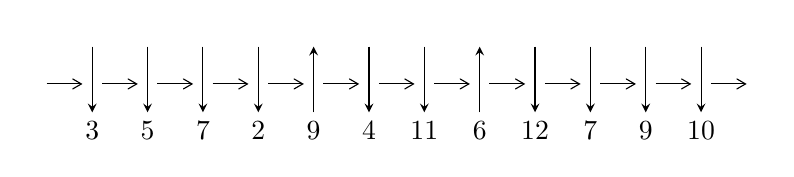
\begin{tikzpicture}[x=20pt, y=17pt]
	% nodes
	\node (C0) at (0, 0) {};
	\node (C1) at (1, 0) {};
	\node (C1U) at (1, +1) {};
	\node (C1D) at (1, -1) {3};

	\node (C2) at (2, 0) {};
	\node (C2U) at (2, +1) {};
	\node (C2D) at (2, -1) {5};

	\node (C3) at (3, 0) {};
	\node (C3U) at (3, +1) {};
	\node (C3D) at (3, -1) {7};

	\node (C4) at (4, 0) {};
	\node (C4U) at (4, +1) {};
	\node (C4D) at (4, -1) {2};

	\node (C5) at (5, 0) {};
	\node (C5U) at (5, +1) {};
	\node (C5D) at (5, -1) {9};

	\node (C6) at (6, 0) {};
	\node (C6U) at (6, +1) {};
	\node (C6D) at (6, -1) {4};

	\node (C7) at (7, 0) {};
	\node (C7U) at (7, +1) {};
	\node (C7D) at (7, -1) {11};

	\node (C8) at (8, 0) {};
	\node (C8U) at (8, +1) {};
	\node (C8D) at (8, -1) {6};

	\node (C9) at (9, 0) {};
	\node (C9U) at (9, +1) {};
	\node (C9D) at (9, -1) {12};

	\node (C10) at (10, 0) {};
	\node (C10U) at (10, +1) {};
	\node (C10D) at (10, -1) {7};

	\node (C11) at (11, 0) {};
	\node (C11U) at (11, +1) {};
	\node (C11D) at (11, -1) {9};

	\node (C12) at (12, 0) {};
	\node (C12U) at (12, +1) {};
	\node (C12D) at (12, -1) {10};
	\node (C13) at (13, 0) {};

	% arrows
	\draw[->,>={angle 60}]
	(C0) edge (C1) (C1) edge (C2) (C2) edge (C3) (C3) edge (C4) (C4) edge (C5) (C5) edge (C6) (C6) edge (C7) (C7) edge (C8) (C8) edge (C9) (C9) edge (C10) (C10) edge (C11) (C11) edge (C12) (C12) edge (C13) ;	\draw[->,>=stealth]
	(C1U) edge (C1D) (C2U) edge (C2D) (C3U) edge (C3D) (C4U) edge (C4D) (C5D) edge (C5U) (C6U) edge (C6D) (C7U) edge (C7D) (C8D) edge (C8U) (C9U) edge (C9D) (C10U) edge (C10D) (C11U) edge (C11D) (C12U) edge (C12D) ;
	\end{tikzpicture} \\
\hhline{~~} \\& 
\textbf{Solving Sequence} \\ \cline{2-2} 
 &
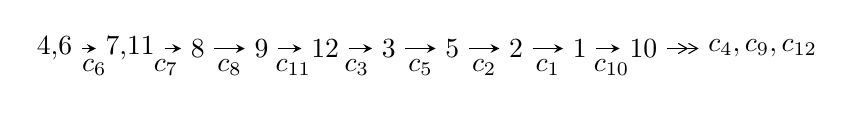
\begin{tikzpicture}[x=23pt, y=7pt]
	% node
	\node (A0) at (-1/8, 0) {4,6};
	\node (A1) at (17/16, 0) {7,11};
	\node (A2) at (17/8, 0) {8};
	\node (A3) at (25/8, 0) {9};
	\node (A4) at (33/8, 0) {12};
	\node (A5) at (41/8, 0) {3};
	\node (A6) at (49/8, 0) {5};
	\node (A7) at (57/8, 0) {2};
	\node (A8) at (65/8, 0) {1};
	\node (A9) at (73/8, 0) {10};
	\node (C1) at (1/2, -1) {$c_{6}$};
	\node (C2) at (13/8, -1) {$c_{7}$};
	\node (C3) at (21/8, -1) {$c_{8}$};
	\node (C4) at (29/8, -1) {$c_{11}$};
	\node (C5) at (37/8, -1) {$c_{3}$};
	\node (C6) at (45/8, -1) {$c_{5}$};
	\node (C7) at (53/8, -1) {$c_{2}$};
	\node (C8) at (61/8, -1) {$c_{1}$};
	\node (C9) at (69/8, -1) {$c_{10}$};
	\node (A10) at (11, 0) {$c_{4},c_{9},c_{12}$};

	% edge
	\draw[->,>=stealth]	
	(A0) edge (A1) (A1) edge (A2) (A2) edge (A3) (A3) edge (A4) (A4) edge (A5) (A5) edge (A6) (A6) edge (A7) (A7) edge (A8) (A8) edge (A9) ;
	\draw[->>,>={angle 60}]	
	(A9) edge (A10);
\end{tikzpicture} \\ 

\end{tabular} \\

\footnotetext{
The image of knot diagram is generated by the software ``\textbf{Draw programme}" developed by Andrew Bartholomew(\url{http://www.layer8.co.uk/maths/draw/index.htm\#Running-draw}), where we modified some parts for our purpose(\url{https://github.com/CATsTAILs/LinksPainter}).
}\phantom \\ \newline 
\centering \textbf{Ideals for irreducible components\footnotemark of $X_{\text{par}}$} 
 
\begin{align*}
I^u_{1}&=\langle 
8.15753\times10^{41} u^{22}-3.72668\times10^{42} u^{21}+\cdots+7.71580\times10^{42} b+1.17939\times10^{43},\\
\phantom{I^u_{1}}&\phantom{= \langle  }1.10388\times10^{43} u^{22}-4.86462\times10^{43} u^{21}+\cdots+1.54316\times10^{43} a+2.96744\times10^{44},\;u^{23}-4 u^{22}+\cdots-36 u+8\rangle \\
I^u_{2}&=\langle 
- u^8+2 u^7-3 u^6+3 u^5-4 u^4+4 u^3-3 u^2+b+2 u-1,\\
\phantom{I^u_{2}}&\phantom{= \langle  }-3 u^8+4 u^7-8 u^6+7 u^5-13 u^4+9 u^3-11 u^2+a+6 u-6,\;u^9- u^8+2 u^7- u^6+3 u^5- u^4+2 u^3+u+1\rangle \\
I^u_{3}&=\langle 
-2 u^2 a- a u- u^2+b- u,\;-2 u^2 a+a^2- a u-11 u^2-2 a-5 u-19,\;u^3+u^2+2 u+1\rangle \\
\\
I^v_{1}&=\langle 
a,\;5 v^2+7 b-49 v+11,\;v^3-10 v^2+5 v-1\rangle \\
\end{align*}
\raggedright * 4 irreducible components of $\dim_{\mathbb{C}}=0$, with total 41 representations.\\
\footnotetext{All coefficients of polynomials are rational numbers. But the coefficients are sometimes approximated in decimal forms when there is not enough margin.}
\newpage
\renewcommand{\arraystretch}{1}
\centering \section*{I. $I^u_{1}= \langle 8.16\times10^{41} u^{22}-3.73\times10^{42} u^{21}+\cdots+7.72\times10^{42} b+1.18\times10^{43},\;1.10\times10^{43} u^{22}-4.86\times10^{43} u^{21}+\cdots+1.54\times10^{43} a+2.97\times10^{44},\;u^{23}-4 u^{22}+\cdots-36 u+8 \rangle$}
\flushleft \textbf{(i) Arc colorings}\\
\begin{tabular}{m{7pt} m{180pt} m{7pt} m{180pt} }
\flushright $a_{4}=$&$\begin{pmatrix}0\\u\end{pmatrix}$ \\
\flushright $a_{6}=$&$\begin{pmatrix}1\\0\end{pmatrix}$ \\
\flushright $a_{7}=$&$\begin{pmatrix}1\\u^2\end{pmatrix}$ \\
\flushright $a_{11}=$&$\begin{pmatrix}-0.715334 u^{22}+3.15238 u^{21}+\cdots+69.0282 u-19.2296\\-0.105725 u^{22}+0.482993 u^{21}+\cdots+14.9531 u-1.52853\end{pmatrix}$ \\
\flushright $a_{8}=$&$\begin{pmatrix}-0.186391 u^{22}+0.803680 u^{21}+\cdots+9.92260 u-5.79288\\-0.0258071 u^{22}+0.120060 u^{21}+\cdots+3.37054 u-0.131649\end{pmatrix}$ \\
\flushright $a_{9}=$&$\begin{pmatrix}-0.212198 u^{22}+0.923740 u^{21}+\cdots+13.2931 u-5.92453\\-0.0258071 u^{22}+0.120060 u^{21}+\cdots+3.37054 u-0.131649\end{pmatrix}$ \\
\flushright $a_{12}=$&$\begin{pmatrix}-0.576767 u^{22}+2.56286 u^{21}+\cdots+55.9572 u-14.4153\\-0.115767 u^{22}+0.522790 u^{21}+\cdots+12.7973 u-1.57836\end{pmatrix}$ \\
\flushright $a_{3}=$&$\begin{pmatrix}u\\u^3+u\end{pmatrix}$ \\
\flushright $a_{5}=$&$\begin{pmatrix}0.0635667 u^{22}-0.259763 u^{21}+\cdots-11.3894 u+1.71111\\0.00786141 u^{22}-0.0482210 u^{21}+\cdots+1.53688 u-0.150885\end{pmatrix}$ \\
\flushright $a_{2}=$&$\begin{pmatrix}-0.0506560 u^{22}+0.189656 u^{21}+\cdots+13.6327 u-1.90596\\0.0232321 u^{22}-0.108930 u^{21}+\cdots+2.18167 u-0.0911079\end{pmatrix}$ \\
\flushright $a_{1}=$&$\begin{pmatrix}-0.0557053 u^{22}+0.211542 u^{21}+\cdots+12.9263 u-1.86199\\0.0193035 u^{22}-0.0931377 u^{21}+\cdots+1.57646 u-0.0606498\end{pmatrix}$ \\
\flushright $a_{10}=$&$\begin{pmatrix}-0.714037 u^{22}+3.15386 u^{21}+\cdots+67.7812 u-18.4298\\-0.108857 u^{22}+0.493167 u^{21}+\cdots+15.1831 u-1.58195\end{pmatrix}$\\&\end{tabular}
\flushleft \textbf{(ii) Obstruction class $= -1$}\\~\\
\flushleft \textbf{(iii) Cusp Shapes $= -4.74869 u^{22}+21.0543 u^{21}+\cdots+605.964 u-98.1244$}\\~\\
\newpage\renewcommand{\arraystretch}{1}
\flushleft \textbf{(iv) u-Polynomials at the component}\newline \\
\begin{tabular}{m{50pt}|m{274pt}}
Crossings & \hspace{64pt}u-Polynomials at each crossing \\
\hline $$\begin{aligned}c_{1}\end{aligned}$$&$\begin{aligned}
&u^{23}+23 u^{22}+\cdots+12783 u+1
\end{aligned}$\\
\hline $$\begin{aligned}c_{2},c_{4}\end{aligned}$$&$\begin{aligned}
&u^{23}-7 u^{22}+\cdots-113 u-1
\end{aligned}$\\
\hline $$\begin{aligned}c_{3},c_{6}\end{aligned}$$&$\begin{aligned}
&u^{23}-4 u^{22}+\cdots-36 u+8
\end{aligned}$\\
\hline $$\begin{aligned}c_{5},c_{8}\end{aligned}$$&$\begin{aligned}
&u^{23}+3 u^{22}+\cdots-32 u-64
\end{aligned}$\\
\hline $$\begin{aligned}c_{7},c_{10}\end{aligned}$$&$\begin{aligned}
&u^{23}+5 u^{22}+\cdots+4608 u-512
\end{aligned}$\\
\hline $$\begin{aligned}c_{9},c_{11},c_{12}\end{aligned}$$&$\begin{aligned}
&u^{23}-14 u^{22}+\cdots+247 u+1
\end{aligned}$\\
\hline
\end{tabular}\\~\\
\newpage\renewcommand{\arraystretch}{1}
\flushleft \textbf{(v) Riley Polynomials at the component}\newline \\
\begin{tabular}{m{50pt}|m{274pt}}
Crossings & \hspace{64pt}Riley Polynomials at each crossing \\
\hline $$\begin{aligned}c_{1}\end{aligned}$$&$\begin{aligned}
&y^{23}-39 y^{22}+\cdots+163240279 y-1
\end{aligned}$\\
\hline $$\begin{aligned}c_{2},c_{4}\end{aligned}$$&$\begin{aligned}
&y^{23}-23 y^{22}+\cdots+12783 y-1
\end{aligned}$\\
\hline $$\begin{aligned}c_{3},c_{6}\end{aligned}$$&$\begin{aligned}
&y^{23}-12 y^{22}+\cdots+7568 y-64
\end{aligned}$\\
\hline $$\begin{aligned}c_{5},c_{8}\end{aligned}$$&$\begin{aligned}
&y^{23}+37 y^{22}+\cdots+234496 y-4096
\end{aligned}$\\
\hline $$\begin{aligned}c_{7},c_{10}\end{aligned}$$&$\begin{aligned}
&y^{23}-111 y^{22}+\cdots+71041024 y-262144
\end{aligned}$\\
\hline $$\begin{aligned}c_{9},c_{11},c_{12}\end{aligned}$$&$\begin{aligned}
&y^{23}-48 y^{22}+\cdots+59963 y-1
\end{aligned}$\\
\hline
\end{tabular}\\~\\
\newpage\flushleft \textbf{(vi) Complex Volumes and Cusp Shapes}
$$\begin{array}{c|c|c}  
\text{Solutions to }I^u_{1}& \I (\text{vol} + \sqrt{-1}CS) & \text{Cusp shape}\\
 \hline 
\begin{aligned}
u &= -0.810706 + 0.505931 I \\
a &= -0.375875 - 0.573416 I \\
b &= -0.094068 - 0.572082 I\end{aligned}
 & -0.87687 + 1.52898 I & -6.60742 - 3.54271 I \\ \hline\begin{aligned}
u &= -0.810706 - 0.505931 I \\
a &= -0.375875 + 0.573416 I \\
b &= -0.094068 + 0.572082 I\end{aligned}
 & -0.87687 - 1.52898 I & -6.60742 + 3.54271 I \\ \hline\begin{aligned}
u &= -0.273102 + 1.253150 I \\
a &= \phantom{-}0.905694 + 0.280329 I \\
b &= -1.78345 - 1.11930 I\end{aligned}
 & \phantom{-}2.20419 + 2.68521 I & \phantom{-}2.70136 + 6.44368 I \\ \hline\begin{aligned}
u &= -0.273102 - 1.253150 I \\
a &= \phantom{-}0.905694 - 0.280329 I \\
b &= -1.78345 + 1.11930 I\end{aligned}
 & \phantom{-}2.20419 - 2.68521 I & \phantom{-}2.70136 - 6.44368 I \\ \hline\begin{aligned}
u &= -0.282905 + 0.561433 I \\
a &= \phantom{-}0.025171 + 0.255386 I \\
b &= \phantom{-}0.116102 - 1.176160 I\end{aligned}
 & \phantom{-}1.45854 + 3.25209 I & -3.51442 - 11.82565 I \\ \hline\begin{aligned}
u &= -0.282905 - 0.561433 I \\
a &= \phantom{-}0.025171 - 0.255386 I \\
b &= \phantom{-}0.116102 + 1.176160 I\end{aligned}
 & \phantom{-}1.45854 - 3.25209 I & -3.51442 + 11.82565 I \\ \hline\begin{aligned}
u &= \phantom{-}0.904186 + 1.051940 I \\
a &= -0.346587 - 0.098446 I \\
b &= -0.141661 + 0.415462 I\end{aligned}
 & -5.12106 - 6.15902 I & -10.50715 + 1.63362 I \\ \hline\begin{aligned}
u &= \phantom{-}0.904186 - 1.051940 I \\
a &= -0.346587 + 0.098446 I \\
b &= -0.141661 - 0.415462 I\end{aligned}
 & -5.12106 + 6.15902 I & -10.50715 - 1.63362 I \\ \hline\begin{aligned}
u &= \phantom{-}0.603575\phantom{ +0.000000I} \\
a &= \phantom{-}4.66294\phantom{ +0.000000I} \\
b &= \phantom{-}0.0529154\phantom{ +0.000000I}\end{aligned}
 & -9.92701\phantom{ +0.000000I} & \phantom{-}35.8110\phantom{ +0.000000I} \\ \hline\begin{aligned}
u &= -0.518673\phantom{ +0.000000I} \\
a &= \phantom{-}1.24139\phantom{ +0.000000I} \\
b &= \phantom{-}0.270054\phantom{ +0.000000I}\end{aligned}
 & -1.19404\phantom{ +0.000000I} & -8.40790\phantom{ +0.000000I}\\
 \hline 
 \end{array}$$\newpage$$\begin{array}{c|c|c}  
\text{Solutions to }I^u_{1}& \I (\text{vol} + \sqrt{-1}CS) & \text{Cusp shape}\\
 \hline 
\begin{aligned}
u &= -0.271589 + 0.441556 I \\
a &= \phantom{-}0.17891 - 4.69126 I \\
b &= -0.423841 + 0.717638 I\end{aligned}
 & -2.85899 + 0.09109 I & -11.2448 - 8.7640 I \\ \hline\begin{aligned}
u &= -0.271589 - 0.441556 I \\
a &= \phantom{-}0.17891 + 4.69126 I \\
b &= -0.423841 - 0.717638 I\end{aligned}
 & -2.85899 - 0.09109 I & -11.2448 + 8.7640 I \\ \hline\begin{aligned}
u &= -0.439625\phantom{ +0.000000I} \\
a &= -12.6495\phantom{ +0.000000I} \\
b &= -2.20680\phantom{ +0.000000I}\end{aligned}
 & -2.87501\phantom{ +0.000000I} & -99.4720\phantom{ +0.000000I} \\ \hline\begin{aligned}
u &= \phantom{-}0.0940545\phantom{ +0.000000I} \\
a &= -7.89489\phantom{ +0.000000I} \\
b &= \phantom{-}0.510696\phantom{ +0.000000I}\end{aligned}
 & -1.10354\phantom{ +0.000000I} & -8.74790\phantom{ +0.000000I} \\ \hline\begin{aligned}
u &= \phantom{-}1.16222 + 1.51464 I \\
a &= -0.789835 + 0.935119 I \\
b &= -0.43899 - 2.10734 I\end{aligned}
 & \phantom{-}15.7088 - 13.9110 I & -11.35191 + 5.40734 I \\ \hline\begin{aligned}
u &= \phantom{-}1.16222 - 1.51464 I \\
a &= -0.789835 - 0.935119 I \\
b &= -0.43899 + 2.10734 I\end{aligned}
 & \phantom{-}15.7088 + 13.9110 I & -11.35191 - 5.40734 I \\ \hline\begin{aligned}
u &= -1.41200 + 1.76863 I \\
a &= -0.536030 - 0.772744 I \\
b &= -0.24550 + 2.28839 I\end{aligned}
 & \phantom{-}19.7178 + 6.1351 I & \phantom{-0.000000 } 0 \\ \hline\begin{aligned}
u &= -1.41200 - 1.76863 I \\
a &= -0.536030 + 0.772744 I \\
b &= -0.24550 - 2.28839 I\end{aligned}
 & \phantom{-}19.7178 - 6.1351 I & \phantom{-0.000000 } 0 \\ \hline\begin{aligned}
u &= \phantom{-}2.39957 + 0.70874 I \\
a &= \phantom{-}0.624715 - 0.384715 I \\
b &= \phantom{-}0.36478 + 1.74735 I\end{aligned}
 & -14.2988 - 3.5584 I & \phantom{-0.000000 } 0 \\ \hline\begin{aligned}
u &= \phantom{-}2.39957 - 0.70874 I \\
a &= \phantom{-}0.624715 + 0.384715 I \\
b &= \phantom{-}0.36478 - 1.74735 I\end{aligned}
 & -14.2988 + 3.5584 I & \phantom{-0.000000 } 0\\
 \hline 
 \end{array}$$\newpage$$\begin{array}{c|c|c}  
\text{Solutions to }I^u_{1}& \I (\text{vol} + \sqrt{-1}CS) & \text{Cusp shape}\\
 \hline 
\begin{aligned}
u &= -2.52063\phantom{ +0.000000I} \\
a &= \phantom{-}0.877307\phantom{ +0.000000I} \\
b &= \phantom{-}0.551360\phantom{ +0.000000I}\end{aligned}
 & \phantom{-}18.9120\phantom{ +0.000000I} & \phantom{-0.000000 } 0 \\ \hline\begin{aligned}
u &= \phantom{-}1.97498 + 1.71262 I \\
a &= -0.304781 + 0.587751 I \\
b &= \phantom{-}0.05752 - 2.27275 I\end{aligned}
 & \phantom{-}14.2364 + 2.5672 I & \phantom{-0.000000 } 0 \\ \hline\begin{aligned}
u &= \phantom{-}1.97498 - 1.71262 I \\
a &= -0.304781 - 0.587751 I \\
b &= \phantom{-}0.05752 + 2.27275 I\end{aligned}
 & \phantom{-}14.2364 - 2.5672 I & \phantom{-0.000000 } 0\\
 \hline 
 \end{array}$$\newpage\newpage\renewcommand{\arraystretch}{1}
\centering \section*{II. $I^u_{2}= \langle - u^8+2 u^7+\cdots+b-1,\;-3 u^8+4 u^7+\cdots+a-6,\;u^9- u^8+2 u^7- u^6+3 u^5- u^4+2 u^3+u+1 \rangle$}
\flushleft \textbf{(i) Arc colorings}\\
\begin{tabular}{m{7pt} m{180pt} m{7pt} m{180pt} }
\flushright $a_{4}=$&$\begin{pmatrix}0\\u\end{pmatrix}$ \\
\flushright $a_{6}=$&$\begin{pmatrix}1\\0\end{pmatrix}$ \\
\flushright $a_{7}=$&$\begin{pmatrix}1\\u^2\end{pmatrix}$ \\
\flushright $a_{11}=$&$\begin{pmatrix}3 u^8-4 u^7+8 u^6-7 u^5+13 u^4-9 u^3+11 u^2-6 u+6\\u^8-2 u^7+3 u^6-3 u^5+4 u^4-4 u^3+3 u^2-2 u+1\end{pmatrix}$ \\
\flushright $a_{8}=$&$\begin{pmatrix}1\\u^2\end{pmatrix}$ \\
\flushright $a_{9}=$&$\begin{pmatrix}u^2+1\\u^2\end{pmatrix}$ \\
\flushright $a_{12}=$&$\begin{pmatrix}3 u^8-4 u^7+8 u^6-7 u^5+13 u^4-9 u^3+10 u^2-6 u+5\\u^8-2 u^7+3 u^6-3 u^5+4 u^4-4 u^3+2 u^2-2 u+1\end{pmatrix}$ \\
\flushright $a_{3}=$&$\begin{pmatrix}u\\u^3+u\end{pmatrix}$ \\
\flushright $a_{5}=$&$\begin{pmatrix}u^4+u^2+1\\u^4\end{pmatrix}$ \\
\flushright $a_{2}=$&$\begin{pmatrix}- u^6- u^4-2 u^2-1\\- u^8-2 u^6-2 u^4-2 u^2\end{pmatrix}$ \\
\flushright $a_{1}=$&$\begin{pmatrix}- u^2-1\\- u^2\end{pmatrix}$ \\
\flushright $a_{10}=$&$\begin{pmatrix}3 u^8-4 u^7+8 u^6-7 u^5+13 u^4-9 u^3+11 u^2-6 u+6\\u^8-2 u^7+3 u^6-3 u^5+4 u^4-4 u^3+3 u^2-2 u+1\end{pmatrix}$\\&\end{tabular}
\flushleft \textbf{(ii) Obstruction class $= 1$}\\~\\
\flushleft \textbf{(iii) Cusp Shapes $= 45 u^8-63 u^7+119 u^6-104 u^5+184 u^4-133 u^3+157 u^2-83 u+73$}\\~\\
\newpage\renewcommand{\arraystretch}{1}
\flushleft \textbf{(iv) u-Polynomials at the component}\newline \\
\begin{tabular}{m{50pt}|m{274pt}}
Crossings & \hspace{64pt}u-Polynomials at each crossing \\
\hline $$\begin{aligned}c_{1}\end{aligned}$$&$\begin{aligned}
&u^9-5 u^8+12 u^7-15 u^6+9 u^5+u^4-4 u^3+2 u^2+u-1
\end{aligned}$\\
\hline $$\begin{aligned}c_{2}\end{aligned}$$&$\begin{aligned}
&u^9+u^8-2 u^7-3 u^6+u^5+3 u^4+2 u^3- u-1
\end{aligned}$\\
\hline $$\begin{aligned}c_{3}\end{aligned}$$&$\begin{aligned}
&u^9+u^8+2 u^7+u^6+3 u^5+u^4+2 u^3+u-1
\end{aligned}$\\
\hline $$\begin{aligned}c_{4}\end{aligned}$$&$\begin{aligned}
&u^9- u^8-2 u^7+3 u^6+u^5-3 u^4+2 u^3- u+1
\end{aligned}$\\
\hline $$\begin{aligned}c_{5}\end{aligned}$$&$\begin{aligned}
&u^9+3 u^8+8 u^7+13 u^6+17 u^5+17 u^4+12 u^3+6 u^2+u-1
\end{aligned}$\\
\hline $$\begin{aligned}c_{6}\end{aligned}$$&$\begin{aligned}
&u^9- u^8+2 u^7- u^6+3 u^5- u^4+2 u^3+u+1
\end{aligned}$\\
\hline $$\begin{aligned}c_{7},c_{10}\end{aligned}$$&$\begin{aligned}
&u^9
\end{aligned}$\\
\hline $$\begin{aligned}c_{8}\end{aligned}$$&$\begin{aligned}
&u^9-3 u^8+8 u^7-13 u^6+17 u^5-17 u^4+12 u^3-6 u^2+u+1
\end{aligned}$\\
\hline $$\begin{aligned}c_{9}\end{aligned}$$&$\begin{aligned}
&(u-1)^9
\end{aligned}$\\
\hline $$\begin{aligned}c_{11},c_{12}\end{aligned}$$&$\begin{aligned}
&(u+1)^9
\end{aligned}$\\
\hline
\end{tabular}\\~\\
\newpage\renewcommand{\arraystretch}{1}
\flushleft \textbf{(v) Riley Polynomials at the component}\newline \\
\begin{tabular}{m{50pt}|m{274pt}}
Crossings & \hspace{64pt}Riley Polynomials at each crossing \\
\hline $$\begin{aligned}c_{1}\end{aligned}$$&$\begin{aligned}
&y^9- y^8+12 y^7-7 y^6+37 y^5+y^4-10 y^2+5 y-1
\end{aligned}$\\
\hline $$\begin{aligned}c_{2},c_{4}\end{aligned}$$&$\begin{aligned}
&y^9-5 y^8+12 y^7-15 y^6+9 y^5+y^4-4 y^3+2 y^2+y-1
\end{aligned}$\\
\hline $$\begin{aligned}c_{3},c_{6}\end{aligned}$$&$\begin{aligned}
&y^9+3 y^8+8 y^7+13 y^6+17 y^5+17 y^4+12 y^3+6 y^2+y-1
\end{aligned}$\\
\hline $$\begin{aligned}c_{5},c_{8}\end{aligned}$$&$\begin{aligned}
&y^9+7 y^8+20 y^7+25 y^6+5 y^5-15 y^4+22 y^2+13 y-1
\end{aligned}$\\
\hline $$\begin{aligned}c_{7},c_{10}\end{aligned}$$&$\begin{aligned}
&y^9
\end{aligned}$\\
\hline $$\begin{aligned}c_{9},c_{11},c_{12}\end{aligned}$$&$\begin{aligned}
&(y-1)^9
\end{aligned}$\\
\hline
\end{tabular}\\~\\
\newpage\flushleft \textbf{(vi) Complex Volumes and Cusp Shapes}
$$\begin{array}{c|c|c}  
\text{Solutions to }I^u_{2}& \I (\text{vol} + \sqrt{-1}CS) & \text{Cusp shape}\\
 \hline 
\begin{aligned}
u &= -0.140343 + 0.966856 I \\
a &= \phantom{-}0.920144 - 0.598375 I \\
b &= -1.004430 + 0.297869 I\end{aligned}
 & \phantom{-}0.13850 + 2.09337 I & -6.65973 - 4.50528 I \\ \hline\begin{aligned}
u &= -0.140343 - 0.966856 I \\
a &= \phantom{-}0.920144 + 0.598375 I \\
b &= -1.004430 - 0.297869 I\end{aligned}
 & \phantom{-}0.13850 - 2.09337 I & -6.65973 + 4.50528 I \\ \hline\begin{aligned}
u &= -0.628449 + 0.875112 I \\
a &= -0.590648 - 0.449402 I \\
b &= -0.275254 + 0.816341 I\end{aligned}
 & -2.26187 + 2.45442 I & -9.69685 - 4.13179 I \\ \hline\begin{aligned}
u &= -0.628449 - 0.875112 I \\
a &= -0.590648 + 0.449402 I \\
b &= -0.275254 - 0.816341 I\end{aligned}
 & -2.26187 - 2.45442 I & -9.69685 + 4.13179 I \\ \hline\begin{aligned}
u &= \phantom{-}0.796005 + 0.733148 I \\
a &= -0.719281 - 0.119276 I \\
b &= \phantom{-}0.070080 - 0.850995 I\end{aligned}
 & -6.01628 + 1.33617 I & -13.00050 - 1.13735 I \\ \hline\begin{aligned}
u &= \phantom{-}0.796005 - 0.733148 I \\
a &= -0.719281 + 0.119276 I \\
b &= \phantom{-}0.070080 + 0.850995 I\end{aligned}
 & -6.01628 - 1.33617 I & -13.00050 + 1.13735 I \\ \hline\begin{aligned}
u &= \phantom{-}0.728966 + 0.986295 I \\
a &= -0.365868 + 0.247975 I \\
b &= -0.195086 - 0.635552 I\end{aligned}
 & -5.24306 - 7.08493 I & -11.6081 + 10.4867 I \\ \hline\begin{aligned}
u &= \phantom{-}0.728966 - 0.986295 I \\
a &= -0.365868 - 0.247975 I \\
b &= -0.195086 + 0.635552 I\end{aligned}
 & -5.24306 + 7.08493 I & -11.6081 - 10.4867 I \\ \hline\begin{aligned}
u &= -0.512358\phantom{ +0.000000I} \\
a &= \phantom{-}14.5113\phantom{ +0.000000I} \\
b &= \phantom{-}3.80937\phantom{ +0.000000I}\end{aligned}
 & -2.84338\phantom{ +0.000000I} & \phantom{-}193.930\phantom{ +0.000000I}\\
 \hline 
 \end{array}$$\newpage\newpage\renewcommand{\arraystretch}{1}
\centering \section*{III. $I^u_{3}= \langle -2 u^2 a- a u- u^2+b- u,\;-2 u^2 a+a^2- a u-11 u^2-2 a-5 u-19,\;u^3+u^2+2 u+1 \rangle$}
\flushleft \textbf{(i) Arc colorings}\\
\begin{tabular}{m{7pt} m{180pt} m{7pt} m{180pt} }
\flushright $a_{4}=$&$\begin{pmatrix}0\\u\end{pmatrix}$ \\
\flushright $a_{6}=$&$\begin{pmatrix}1\\0\end{pmatrix}$ \\
\flushright $a_{7}=$&$\begin{pmatrix}1\\u^2\end{pmatrix}$ \\
\flushright $a_{11}=$&$\begin{pmatrix}a\\2 u^2 a+a u+u^2+u\end{pmatrix}$ \\
\flushright $a_{8}=$&$\begin{pmatrix}- u^2 a- a u-3 u^2- a-2 u-4\\0\end{pmatrix}$ \\
\flushright $a_{9}=$&$\begin{pmatrix}- u^2 a- a u-3 u^2- a-2 u-4\\0\end{pmatrix}$ \\
\flushright $a_{12}=$&$\begin{pmatrix}-2 u^2 a-2 a u-4 u^2- a-3 u-5\\2 u^2 a+a u+u^2+u\end{pmatrix}$ \\
\flushright $a_{3}=$&$\begin{pmatrix}u\\- u^2- u-1\end{pmatrix}$ \\
\flushright $a_{5}=$&$\begin{pmatrix}1\\0\end{pmatrix}$ \\
\flushright $a_{2}=$&$\begin{pmatrix}- u^2-1\\- u^2- u-1\end{pmatrix}$ \\
\flushright $a_{1}=$&$\begin{pmatrix}-1\\- u^2\end{pmatrix}$ \\
\flushright $a_{10}=$&$\begin{pmatrix}u^2 a+a u+u^2+a+u\\- u^2\end{pmatrix}$\\&\end{tabular}
\flushleft \textbf{(ii) Obstruction class $= 1$}\\~\\
\flushleft \textbf{(iii) Cusp Shapes $= -12 u^2 a-21 u^2-3 a-13 u-44$}\\~\\
\newpage\renewcommand{\arraystretch}{1}
\flushleft \textbf{(iv) u-Polynomials at the component}\newline \\
\begin{tabular}{m{50pt}|m{274pt}}
Crossings & \hspace{64pt}u-Polynomials at each crossing \\
\hline $$\begin{aligned}c_{1},c_{3}\end{aligned}$$&$\begin{aligned}
&(u^3- u^2+2 u-1)^2
\end{aligned}$\\
\hline $$\begin{aligned}c_{2}\end{aligned}$$&$\begin{aligned}
&(u^3+u^2-1)^2
\end{aligned}$\\
\hline $$\begin{aligned}c_{4}\end{aligned}$$&$\begin{aligned}
&(u^3- u^2+1)^2
\end{aligned}$\\
\hline $$\begin{aligned}c_{5},c_{8}\end{aligned}$$&$\begin{aligned}
&u^6
\end{aligned}$\\
\hline $$\begin{aligned}c_{6}\end{aligned}$$&$\begin{aligned}
&(u^3+u^2+2 u+1)^2
\end{aligned}$\\
\hline $$\begin{aligned}c_{7},c_{9}\end{aligned}$$&$\begin{aligned}
&(u^2+u-1)^3
\end{aligned}$\\
\hline $$\begin{aligned}c_{10},c_{11},c_{12}\end{aligned}$$&$\begin{aligned}
&(u^2- u-1)^3
\end{aligned}$\\
\hline
\end{tabular}\\~\\
\newpage\renewcommand{\arraystretch}{1}
\flushleft \textbf{(v) Riley Polynomials at the component}\newline \\
\begin{tabular}{m{50pt}|m{274pt}}
Crossings & \hspace{64pt}Riley Polynomials at each crossing \\
\hline $$\begin{aligned}c_{1},c_{3},c_{6}\end{aligned}$$&$\begin{aligned}
&(y^3+3 y^2+2 y-1)^2
\end{aligned}$\\
\hline $$\begin{aligned}c_{2},c_{4}\end{aligned}$$&$\begin{aligned}
&(y^3- y^2+2 y-1)^2
\end{aligned}$\\
\hline $$\begin{aligned}c_{5},c_{8}\end{aligned}$$&$\begin{aligned}
&y^6
\end{aligned}$\\
\hline $$\begin{aligned}c_{7},c_{9},c_{10}\\c_{11},c_{12}\end{aligned}$$&$\begin{aligned}
&(y^2-3 y+1)^3
\end{aligned}$\\
\hline
\end{tabular}\\~\\
\newpage\flushleft \textbf{(vi) Complex Volumes and Cusp Shapes}
$$\begin{array}{c|c|c}  
\text{Solutions to }I^u_{3}& \I (\text{vol} + \sqrt{-1}CS) & \text{Cusp shape}\\
 \hline 
\begin{aligned}
u &= -0.215080 + 1.307140 I \\
a &= -1.284420 - 0.112842 I \\
b &= \phantom{-}2.68975 + 0.90979 I\end{aligned}
 & \phantom{-}2.03717 + 2.82812 I & -27.3018 - 15.7639 I \\ \hline\begin{aligned}
u &= -0.215080 + 1.307140 I \\
a &= -0.255377 + 0.295424 I \\
b &= -1.027390 - 0.347508 I\end{aligned}
 & -5.85852 + 2.82812 I & -12.61597 - 1.90115 I \\ \hline\begin{aligned}
u &= -0.215080 - 1.307140 I \\
a &= -1.284420 + 0.112842 I \\
b &= \phantom{-}2.68975 - 0.90979 I\end{aligned}
 & \phantom{-}2.03717 - 2.82812 I & -27.3018 + 15.7639 I \\ \hline\begin{aligned}
u &= -0.215080 - 1.307140 I \\
a &= -0.255377 - 0.295424 I \\
b &= -1.027390 + 0.347508 I\end{aligned}
 & -5.85852 - 2.82812 I & -12.61597 + 1.90115 I \\ \hline\begin{aligned}
u &= -0.569840\phantom{ +0.000000I} \\
a &= -3.52133\phantom{ +0.000000I} \\
b &= -0.525405\phantom{ +0.000000I}\end{aligned}
 & -2.10041\phantom{ +0.000000I} & -19.1260\phantom{ +0.000000I} \\ \hline\begin{aligned}
u &= -0.569840\phantom{ +0.000000I} \\
a &= \phantom{-}5.60092\phantom{ +0.000000I} \\
b &= \phantom{-}0.200687\phantom{ +0.000000I}\end{aligned}
 & -9.99610\phantom{ +0.000000I} & -82.0390\phantom{ +0.000000I}\\
 \hline 
 \end{array}$$\newpage\newpage\renewcommand{\arraystretch}{1}
\centering \section*{IV. $I^v_{1}= \langle a,\;5 v^2+7 b-49 v+11,\;v^3-10 v^2+5 v-1 \rangle$}
\flushleft \textbf{(i) Arc colorings}\\
\begin{tabular}{m{7pt} m{180pt} m{7pt} m{180pt} }
\flushright $a_{4}=$&$\begin{pmatrix}v\\0\end{pmatrix}$ \\
\flushright $a_{6}=$&$\begin{pmatrix}1\\0\end{pmatrix}$ \\
\flushright $a_{7}=$&$\begin{pmatrix}1\\0\end{pmatrix}$ \\
\flushright $a_{11}=$&$\begin{pmatrix}0\\-\frac{5}{7} v^2+7 v-\frac{11}{7}\end{pmatrix}$ \\
\flushright $a_{8}=$&$\begin{pmatrix}1\\-\frac{2}{7} v^2+3 v-\frac{17}{7}\end{pmatrix}$ \\
\flushright $a_{9}=$&$\begin{pmatrix}-\frac{2}{7} v^2+3 v-\frac{10}{7}\\-\frac{2}{7} v^2+3 v-\frac{17}{7}\end{pmatrix}$ \\
\flushright $a_{12}=$&$\begin{pmatrix}-1\\-\frac{2}{7} v^2+3 v-\frac{17}{7}\end{pmatrix}$ \\
\flushright $a_{3}=$&$\begin{pmatrix}v\\0\end{pmatrix}$ \\
\flushright $a_{5}=$&$\begin{pmatrix}\frac{5}{7} v^2-7 v+\frac{25}{7}\\v^2-10 v+5\end{pmatrix}$ \\
\flushright $a_{2}=$&$\begin{pmatrix}-\frac{5}{7} v^2+8 v-\frac{25}{7}\\- v^2+10 v-5\end{pmatrix}$ \\
\flushright $a_{1}=$&$\begin{pmatrix}-\frac{5}{7} v^2+7 v-\frac{25}{7}\\- v^2+10 v-5\end{pmatrix}$ \\
\flushright $a_{10}=$&$\begin{pmatrix}-\frac{5}{7} v^2+7 v-\frac{11}{7}\\-\frac{5}{7} v^2+7 v-\frac{11}{7}\end{pmatrix}$\\&\end{tabular}
\flushleft \textbf{(ii) Obstruction class $= 1$}\\~\\
\flushleft \textbf{(iii) Cusp Shapes $= \frac{30}{7} v^2-33 v+\frac{3}{7}$}\\~\\
\newpage\renewcommand{\arraystretch}{1}
\flushleft \textbf{(iv) u-Polynomials at the component}\newline \\
\begin{tabular}{m{50pt}|m{274pt}}
Crossings & \hspace{64pt}u-Polynomials at each crossing \\
\hline $$\begin{aligned}c_{1},c_{2}\end{aligned}$$&$\begin{aligned}
&(u-1)^3
\end{aligned}$\\
\hline $$\begin{aligned}c_{3},c_{6}\end{aligned}$$&$\begin{aligned}
&u^3
\end{aligned}$\\
\hline $$\begin{aligned}c_{4}\end{aligned}$$&$\begin{aligned}
&(u+1)^3
\end{aligned}$\\
\hline $$\begin{aligned}c_{5}\end{aligned}$$&$\begin{aligned}
&u^3+3 u^2+2 u-1
\end{aligned}$\\
\hline $$\begin{aligned}c_{7}\end{aligned}$$&$\begin{aligned}
&u^3- u^2+2 u-1
\end{aligned}$\\
\hline $$\begin{aligned}c_{8}\end{aligned}$$&$\begin{aligned}
&u^3-3 u^2+2 u+1
\end{aligned}$\\
\hline $$\begin{aligned}c_{9}\end{aligned}$$&$\begin{aligned}
&u^3+u^2-1
\end{aligned}$\\
\hline $$\begin{aligned}c_{10}\end{aligned}$$&$\begin{aligned}
&u^3+u^2+2 u+1
\end{aligned}$\\
\hline $$\begin{aligned}c_{11},c_{12}\end{aligned}$$&$\begin{aligned}
&u^3- u^2+1
\end{aligned}$\\
\hline
\end{tabular}\\~\\
\newpage\renewcommand{\arraystretch}{1}
\flushleft \textbf{(v) Riley Polynomials at the component}\newline \\
\begin{tabular}{m{50pt}|m{274pt}}
Crossings & \hspace{64pt}Riley Polynomials at each crossing \\
\hline $$\begin{aligned}c_{1},c_{2},c_{4}\end{aligned}$$&$\begin{aligned}
&(y-1)^3
\end{aligned}$\\
\hline $$\begin{aligned}c_{3},c_{6}\end{aligned}$$&$\begin{aligned}
&y^3
\end{aligned}$\\
\hline $$\begin{aligned}c_{5},c_{8}\end{aligned}$$&$\begin{aligned}
&y^3-5 y^2+10 y-1
\end{aligned}$\\
\hline $$\begin{aligned}c_{7},c_{10}\end{aligned}$$&$\begin{aligned}
&y^3+3 y^2+2 y-1
\end{aligned}$\\
\hline $$\begin{aligned}c_{9},c_{11},c_{12}\end{aligned}$$&$\begin{aligned}
&y^3- y^2+2 y-1
\end{aligned}$\\
\hline
\end{tabular}\\~\\
\newpage\flushleft \textbf{(vi) Complex Volumes and Cusp Shapes}
$$\begin{array}{c|c|c}  
\text{Solutions to }I^v_{1}& \I (\text{vol} + \sqrt{-1}CS) & \text{Cusp shape}\\
 \hline 
\begin{aligned}
v &= \phantom{-}0.258045 + 0.197115 I \\
a &= \phantom{-0.000000 } 0 \\
b &= \phantom{-}0.215080 + 1.307140 I\end{aligned}
 & \phantom{-}1.37919 - 2.82812 I & -7.96807 - 6.06881 I \\ \hline\begin{aligned}
v &= \phantom{-}0.258045 - 0.197115 I \\
a &= \phantom{-0.000000 } 0 \\
b &= \phantom{-}0.215080 - 1.307140 I\end{aligned}
 & \phantom{-}1.37919 + 2.82812 I & -7.96807 + 6.06881 I \\ \hline\begin{aligned}
v &= \phantom{-}9.48391\phantom{ +0.000000I} \\
a &= \phantom{-0.000000 } 0 \\
b &= \phantom{-}0.569840\phantom{ +0.000000I}\end{aligned}
 & -2.75839\phantom{ +0.000000I} & \phantom{-}72.9360\phantom{ +0.000000I}\\
 \hline 
 \end{array}$$\newpage
\newpage\renewcommand{\arraystretch}{1}
\centering \section*{ V. u-Polynomials}
\begin{tabular}{m{50pt}|m{274pt}}
Crossings & \hspace{64pt}u-Polynomials at each crossing \\
\hline $$\begin{aligned}c_{1}\end{aligned}$$&$\begin{aligned}
&(u-1)^3(u^3- u^2+2 u-1)^2\\
&\cdot(u^9-5 u^8+12 u^7-15 u^6+9 u^5+u^4-4 u^3+2 u^2+u-1)\\
&\cdot(u^{23}+23 u^{22}+\cdots+12783 u+1)
\end{aligned}$\\
\hline $$\begin{aligned}c_{2}\end{aligned}$$&$\begin{aligned}
&(u-1)^3(u^3+u^2-1)^2(u^9+u^8-2 u^7-3 u^6+u^5+3 u^4+2 u^3- u-1)\\
&\cdot(u^{23}-7 u^{22}+\cdots-113 u-1)
\end{aligned}$\\
\hline $$\begin{aligned}c_{3}\end{aligned}$$&$\begin{aligned}
&u^3(u^3- u^2+2 u-1)^2(u^9+u^8+2 u^7+u^6+3 u^5+u^4+2 u^3+u-1)\\
&\cdot(u^{23}-4 u^{22}+\cdots-36 u+8)
\end{aligned}$\\
\hline $$\begin{aligned}c_{4}\end{aligned}$$&$\begin{aligned}
&(u+1)^3(u^3- u^2+1)^2(u^9- u^8-2 u^7+3 u^6+u^5-3 u^4+2 u^3- u+1)\\
&\cdot(u^{23}-7 u^{22}+\cdots-113 u-1)
\end{aligned}$\\
\hline $$\begin{aligned}c_{5}\end{aligned}$$&$\begin{aligned}
&u^6(u^3+3 u^2+2 u-1)\\
&\cdot(u^9+3 u^8+8 u^7+13 u^6+17 u^5+17 u^4+12 u^3+6 u^2+u-1)\\
&\cdot(u^{23}+3 u^{22}+\cdots-32 u-64)
\end{aligned}$\\
\hline $$\begin{aligned}c_{6}\end{aligned}$$&$\begin{aligned}
&u^3(u^3+u^2+2 u+1)^2(u^9- u^8+2 u^7- u^6+3 u^5- u^4+2 u^3+u+1)\\
&\cdot(u^{23}-4 u^{22}+\cdots-36 u+8)
\end{aligned}$\\
\hline $$\begin{aligned}c_{7}\end{aligned}$$&$\begin{aligned}
&u^9(u^2+u-1)^3(u^3- u^2+2 u-1)(u^{23}+5 u^{22}+\cdots+4608 u-512)
\end{aligned}$\\
\hline $$\begin{aligned}c_{8}\end{aligned}$$&$\begin{aligned}
&u^6(u^3-3 u^2+2 u+1)\\
&\cdot(u^9-3 u^8+8 u^7-13 u^6+17 u^5-17 u^4+12 u^3-6 u^2+u+1)\\
&\cdot(u^{23}+3 u^{22}+\cdots-32 u-64)
\end{aligned}$\\
\hline $$\begin{aligned}c_{9}\end{aligned}$$&$\begin{aligned}
&((u-1)^9)(u^2+u-1)^3(u^3+u^2-1)(u^{23}-14 u^{22}+\cdots+247 u+1)
\end{aligned}$\\
\hline $$\begin{aligned}c_{10}\end{aligned}$$&$\begin{aligned}
&u^9(u^2- u-1)^3(u^3+u^2+2 u+1)(u^{23}+5 u^{22}+\cdots+4608 u-512)
\end{aligned}$\\
\hline $$\begin{aligned}c_{11},c_{12}\end{aligned}$$&$\begin{aligned}
&((u+1)^9)(u^2- u-1)^3(u^3- u^2+1)(u^{23}-14 u^{22}+\cdots+247 u+1)
\end{aligned}$\\
\hline
\end{tabular}\newpage\renewcommand{\arraystretch}{1}
\centering \section*{ VI. Riley Polynomials}
\begin{tabular}{m{50pt}|m{274pt}}
Crossings & \hspace{64pt}Riley Polynomials at each crossing \\
\hline $$\begin{aligned}c_{1}\end{aligned}$$&$\begin{aligned}
&(y-1)^3(y^3+3 y^2+2 y-1)^2\\
&\cdot(y^9- y^8+12 y^7-7 y^6+37 y^5+y^4-10 y^2+5 y-1)\\
&\cdot(y^{23}-39 y^{22}+\cdots+163240279 y-1)
\end{aligned}$\\
\hline $$\begin{aligned}c_{2},c_{4}\end{aligned}$$&$\begin{aligned}
&(y-1)^3(y^3- y^2+2 y-1)^2\\
&\cdot(y^9-5 y^8+12 y^7-15 y^6+9 y^5+y^4-4 y^3+2 y^2+y-1)\\
&\cdot(y^{23}-23 y^{22}+\cdots+12783 y-1)
\end{aligned}$\\
\hline $$\begin{aligned}c_{3},c_{6}\end{aligned}$$&$\begin{aligned}
&y^3(y^3+3 y^2+2 y-1)^2\\
&\cdot(y^9+3 y^8+8 y^7+13 y^6+17 y^5+17 y^4+12 y^3+6 y^2+y-1)\\
&\cdot(y^{23}-12 y^{22}+\cdots+7568 y-64)
\end{aligned}$\\
\hline $$\begin{aligned}c_{5},c_{8}\end{aligned}$$&$\begin{aligned}
&y^6(y^3-5 y^2+10 y-1)\\
&\cdot(y^9+7 y^8+20 y^7+25 y^6+5 y^5-15 y^4+22 y^2+13 y-1)\\
&\cdot(y^{23}+37 y^{22}+\cdots+234496 y-4096)
\end{aligned}$\\
\hline $$\begin{aligned}c_{7},c_{10}\end{aligned}$$&$\begin{aligned}
&y^9(y^2-3 y+1)^3(y^3+3 y^2+2 y-1)\\
&\cdot(y^{23}-111 y^{22}+\cdots+71041024 y-262144)
\end{aligned}$\\
\hline $$\begin{aligned}c_{9},c_{11},c_{12}\end{aligned}$$&$\begin{aligned}
&(y-1)^9(y^2-3 y+1)^3(y^3- y^2+2 y-1)\\
&\cdot(y^{23}-48 y^{22}+\cdots+59963 y-1)
\end{aligned}$\\
\hline
\end{tabular}
\vskip 2pc
\end{document}